% !TeX root = ../main.tex

\chapter{FFmpeg}

\section{FFmpeg简介}

\subsection{FFmpeg 基本组成}

FFmpeg是领先的多媒体框架,“FF”表示“Fast Forward”。FFmpeg 基本组成包含 libavformat,libavcodec,libavfilter,libavdevice,libavutil,libswresample,libswscale 等模块库。
libavformat 库能够实现视频格式封装,解封装和转封装,包含了大多数媒体封装格式,如 MP4,FLV,KV,TS 等文件封装格式,还有 RTMP,RTSP,MMS,HLS 等网络协议封装格式。
libavcodec 库能够实现视频编码,解码和转码,包含了常用的编解码格式,如 MPEG4,AAC,MJPEG 等。
libavfilter 库实现了非常强大的的音视频滤镜功能,可用于多媒体后期的处理与编辑,如添加水印,绿幕抠图,视频裁剪、截图等。
libavdevice 是一个包含输入和输出设备的库,可以从常见的媒体输入框架读取数据并将数据渲染到媒体输出框架中。
libavutil 库包含了很多简化实用工具,其中包括随机数生成器,数据结构,核心多媒体实用程序等。
libswscale 库能够实现图像格式转换,如图像缩放和像素格式转换。
libswresample 库提供了高级别的音频重采样API。

\begin{figure}[h]
\centering
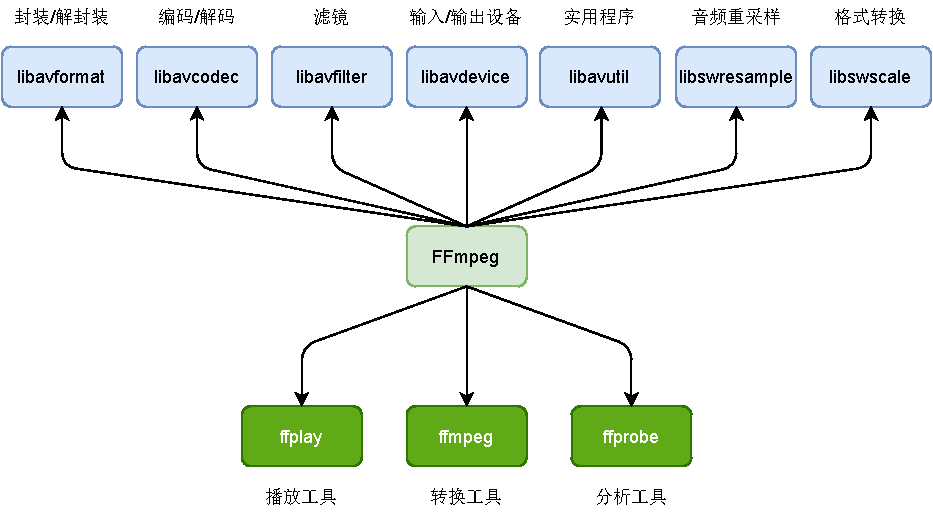
\includegraphics[width=1\textwidth]{ffmpeg.pdf}
\caption{FFmpeg 基本组成}
\label{fig:FFmpeg}
% \note{注:图注的内容不宜放到图题中。}
\end{figure}

FFmpeg 有着强大的跨平台特性,可以在 Linux,Mac OS X,Microsoft Windows 等平台下编译。
编译后会产生上面提到的七个库文件和三种工具。三种工具分别是ffmpeg,ffprobe,ffplay。
其中,ffmpeg 是多媒体处理工具,可以进行视频转码和转封装,ffprobe 是多媒体信息查看工具,fflay 则是一个简单播放器。

% \subsection{ffplay 与 SDL}

% ffplay 是一个简单播放器,使用 FFmpeg 提供的解码器和 SDL(Simple DirectMedia Layer)库进行视频播放。
% SDL 是开源的跨平台开发库,使用C语言编写,旨在通过 OpenGL 和 Direct3D 提供对音频和图形底层硬件的访问。
% SDL 提供了多种控制图像、声音、输入输出的接口,开发者可以使用 SDL 轻易在不同平台(Linux、Windows、Mac OS X等)快速构建音视频处理软件,而无需关心
% 不同平台底层系统的区别。许多视频播放软件,仿真器和游戏都在使用SDL。
% 为了实现跨平台特性,SDL 重新封装了不同操作系统的底层处理库。

% \begin{figure}[h]
% \centering
% 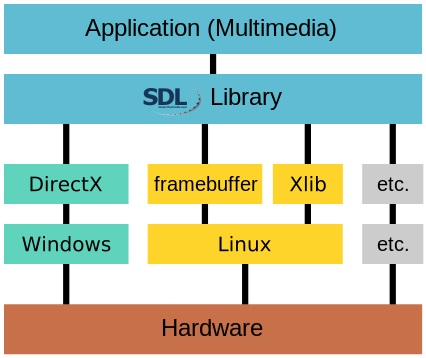
\includegraphics[width=0.5\textwidth]{sdl.jpg}
% \caption{SDL结构}
% \label{fig:sdl}
% % \note{注:图注的内容不宜放到图题中。}
% \end{figure}

\section{ffplay工作流程}

\subsection{解码}

ffplay 使用多线程进行工作,其中一个是读进程,还有三个分别是视频、音频、字幕线程。
如图 \ref{fig:decode} 所示,读进程(read\_thread())首先对视频文件进行解封装,并找到
媒体流信息,然后循环调用 av\_read\_frame() 
获取压缩编码数据 av\_packet,并调用 packet\_queue\_put() 根据编码数据类型的不同(视频、音频、字幕),将 av\_packet 放到对应的 packet\_queue 
中。视频线程主要有两个函数,get\_video\_frame() 和 queue\_picture()。
前者调用 packet\_queue\_get() 从 packet\_queue 中取出压缩编码数据,并使用 libavcodec 库进行解码,然后再调用 avcodec\_receive\_frame()
接收解码后的帧,后者负责把接收到的帧加入到队列。

\begin{figure}[h]
\centering
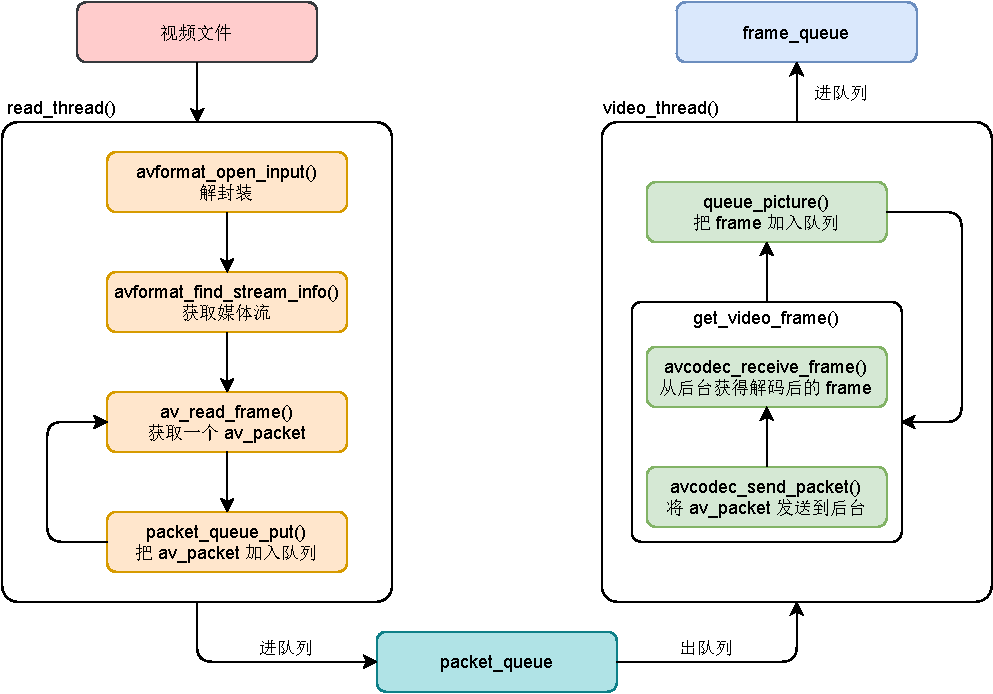
\includegraphics[width=1\textwidth]{decode_1.pdf}
\caption{视频解码流程}
\label{fig:decode}
% \note{注:图中仅画出读进程和视频进程,未体现音频和字幕线程。}
\end{figure}

\subsection{播放}

ffplay 调用 video\_display() 进行视频播放,核心流程如图 \ref{fig:display} 所示。video\_display() 首先调用 SDL\_RenderClean() 清空渲染器,然后进入 video\_image\_display()
函数内部。frame\_queue\_peek\_last() 从解码得到的帧队列中获取帧数据。calculate\_display\_rect() 计算播放窗口的大小,以保证窗口被拉伸时,视频依旧保证纵横比。
upload\_texture() 负责把视频帧的像素数据更新到纹理区域。SDL\_RenderCopy() 则是把纹理数据复制到渲染器中。最后 SDL\_RenderPresent() 将渲染器中的
内容在播放窗口中显示。

\begin{figure}[h]
\centering
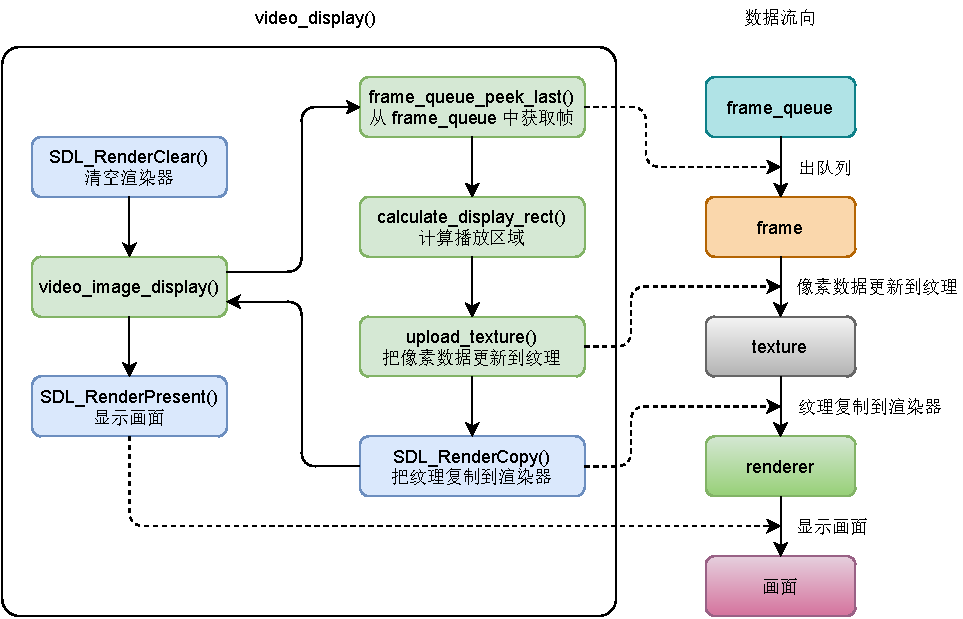
\includegraphics[width=1\textwidth]{display_2.pdf}
\caption{视频播放流程}
\label{fig:display}
% \note{注:图注的内容不宜放到图题中。}
\end{figure}
